\documentclass[conference]{IEEEtran}

\usepackage{amsmath,amssymb,amsfonts}
\usepackage{graphicx}
\graphicspath{{figures/}{./}}
\usepackage{textcomp}
\usepackage{xcolor}
\usepackage{cite}
\usepackage{hyperref}
\usepackage{booktabs}
\usepackage{multirow}

\begin{document}

\title{Evaluating Invariant Extended Kalman Filter Performance for Unmanned Surface Vessel State Estimation Under Varying Sea Conditions}

\author{
  \IEEEauthorblockN{Arvind Madhu Kutirakulam}
  \IEEEauthorblockA{University of Michigan\\Ann Arbor, MI\\akutira@umich.edu}
  \and
  \IEEEauthorblockN{Campbell Taylor}
  \IEEEauthorblockA{University of Michigan\\Ann Arbor, MI\\camtay@umich.edu}
  \and
  \IEEEauthorblockN{Shuai Xu}
  \IEEEauthorblockA{University of Michigan\\Ann Arbor, MI\\shuaixu@umich.edu}
}

\maketitle

% ============================================================
\begin{abstract}
Unmanned Surface Vessels (USVs) increasingly rely on inertial navigation systems (INS) for state estimation, yet heavy sea states can degrade INS accuracy through aggressive vessel motions and sensor drift. This paper presents an empirical comparison of three state estimation approaches for USVs: a standard Extended Kalman Filter (EKF), an Error-State EKF (ES-EKF), and an Invariant Extended Kalman Filter (In-EKF). We evaluate each filter across calm, medium, and high-sea-state scenarios drawn from the KTOE offshore-platform dataset, sampled at 10\,Hz with GPS disabled to isolate INS-only performance. The ES-EKF reduces position RMSE by 15--27\% over the standard EKF across all scenarios, while the In-EKF dominates in the high-seas regime, cutting terminal drift from 116\,m (EKF) to 16\,m --- roughly a seven-fold improvement. Our results demonstrate how estimation error scales with disturbance intensity and highlight the robustness advantages of geometry-aware filtering on the matrix Lie group $SE_2(3)$ for marine navigation.
\end{abstract}

\begin{IEEEkeywords}
state estimation, extended Kalman filter, invariant EKF, unmanned surface vessel, inertial navigation, sea state
\end{IEEEkeywords}

% ============================================================
\section{Introduction}
\label{sec:intro}

Unmanned Surface Vessels (USVs) are a rapidly growing segment of the global small craft fleet, with applications spanning environmental monitoring, maritime security, and oceanographic research. Reliable state estimation---accurately knowing position, velocity, and orientation---is fundamental to autonomous USV operation.

Most USV navigation systems fuse Global Positioning System (GPS) data with Inertial Navigation System (INS) measurements via Kalman filtering techniques~\cite{hawaii_usv}. However, GPS signals may be unavailable or degraded in contested or remote environments, forcing greater reliance on INS alone.

A key concern in INS-dominant operation is that heavy sea states---characterized by large, high-frequency wave motions---may accelerate sensor drift and degrade estimation accuracy beyond levels observed in calm testing conditions. This motivates the central question of our work:

\emph{How does estimation error scale with sea state severity, and can geometry-aware filters such as the Invariant EKF (In-EKF) maintain robustness where standard approaches degrade?}

Our contributions are:
\begin{enumerate}
  \item The evaluation of EKF models on an empirical dataset with variable sea states and ocean conditions.
  \item Implementation and comparison of standard EKF, Error-State EKF, and In-EKF for the USV navigation problem.
  \item Quantitative analysis of estimation error scaling with disturbance intensity.
\end{enumerate}

\paragraph*{Code and video}
All code, data-loading utilities, and plotting scripts used to produce the results in this paper are released as open source at \url{https://github.com/CamumichProject/UofMNA568Gproject}. A video presentation of the project is available at \url{https://youtu.be/vlhaLs5fJts}.

% ============================================================
\section{Related Work}
\label{sec:related}

Kalman filtering has been widely applied to marine vehicle navigation. Early work focused on fusing GPS and INS measurements for surface vessels, demonstrating effective position estimation in calm conditions~\cite{hawaii_usv}.

The Invariant Extended Kalman Filter was introduced by Barrau and Bonnabel~\cite{barrau2017invariant}, exploiting Lie group symmetry in the estimation error to achieve improved convergence and consistency properties. While In-EKF has been validated for ground robots and aerial vehicles, its application to USVs operating in high sea states remains relatively unexplored.

Sea state modeling typically employs standard wave spectra (e.g., Pierson--Moskowitz, JONSWAP) to characterize ocean surface disturbances~\cite{fossen2011handbook}. The interaction between wave-induced vessel motion and INS drift is a known concern but has received limited quantitative treatment in the filtering literature. To help address this gap, we evaluate the filters on empirical data from the KTOE dataset.

% ============================================================
\section{Problem Formulation}
\label{sec:problem}

\subsection{USV State and Dynamics}

We model the USV as a rigid body in full 6-DOF. The filter state is 9-dimensional:
\begin{equation}
  \mathbf{x} = \begin{bmatrix} \mathbf{p}^\top & \mathbf{v}^\top & \boldsymbol{\theta}^\top \end{bmatrix}^\top \in \mathbb{R}^9,
  \label{eq:state}
\end{equation}
where $\mathbf{p} \in \mathbb{R}^3$ is world-frame position (m), $\mathbf{v} \in \mathbb{R}^3$ is world-frame linear velocity (m/s), and $\boldsymbol{\theta} = (\phi, \theta, \psi)$ are the body-to-world Euler angles in the ZYX convention (rad).

The body-to-world rotation is $\mathbf{R}(\boldsymbol{\theta}) \in SO(3)$. The continuous-time dynamics driven by a strapdown IMU-like input $\mathbf{u} = [\mathbf{a}_b^\top\ \boldsymbol{\omega}_b^\top]^\top$ (body-frame linear and angular rates) are:
\begin{equation}
  \dot{\mathbf{p}} = \mathbf{v}, \quad
  \dot{\mathbf{v}} = \mathbf{R}(\boldsymbol{\theta})\,\mathbf{a}_b, \quad
  \dot{\boldsymbol{\theta}} = \boldsymbol{\omega}_b,
  \label{eq:dynamics}
\end{equation}
where the gravity vector is assumed to have been compensated at the IMU level, consistent with the KTOE dataset convention in which the published accelerations are reported relative to the platform's quasi-static equilibrium. These dynamics are integrated with a first-order Euler step of size $\Delta t = 0.1$\,s to match the 10\,Hz dataset cadence:
\begin{equation}
  \mathbf{x}_{k+1} = f(\mathbf{x}_k,\mathbf{u}_k) + \mathbf{w}_k, \quad
  \mathbf{w}_k \sim \mathcal{N}(\mathbf{0}, \mathbf{Q}).
  \label{eq:process}
\end{equation}

\subsection{Measurement Models}

The on-board body-velocity sensor (e.g.\ a Doppler velocity log) supplies body-frame linear velocities $\mathbf{v}_b$ and angular rates $\boldsymbol{\omega}_b$:
\begin{equation}
  \mathbf{z}_k = \begin{bmatrix} \mathbf{R}(\boldsymbol{\theta}_k)^\top \mathbf{v}_k \\ \boldsymbol{\omega}_{b,k} \end{bmatrix} + \mathbf{n}_k,
  \quad \mathbf{n}_k \sim \mathcal{N}(\mathbf{0}, \mathbf{R}),
  \label{eq:meas}
\end{equation}
so that the first three channels are body-frame linear velocity (a nonlinear function of the orientation state) and the last three are angular rate. GPS is intentionally omitted to stress-test INS-only performance as motivated in Section~\ref{sec:intro}.


% ============================================================
\section{Approach}
\label{sec:approach}

\subsection{Standard EKF Baseline}

The standard EKF propagates the 9-D mean state of~\eqref{eq:state} through the nonlinear dynamics~\eqref{eq:dynamics} and linearizes about the current estimate via the process Jacobian $\mathbf{F}_k = \left.\partial f/\partial \mathbf{x}\right|_{\hat{\mathbf{x}}_k,\mathbf{u}_k}$ and the measurement Jacobian $\mathbf{H}_k = \left.\partial h/\partial \mathbf{x}\right|_{\hat{\mathbf{x}}_k}$. Both Jacobians are computed by finite differences, which keeps the baseline robust to tuning of the dynamics. The predict--update recursion is the textbook form:
\begin{align}
  \hat{\mathbf{x}}_{k|k-1} &= f(\hat{\mathbf{x}}_{k-1|k-1}, \mathbf{u}_k) \\
  \mathbf{P}_{k|k-1} &= \mathbf{F}_k \mathbf{P}_{k-1|k-1} \mathbf{F}_k^\top + \mathbf{Q}(\Delta t) \\
  \mathbf{K}_k &= \mathbf{P}_{k|k-1} \mathbf{H}_k^\top (\mathbf{H}_k \mathbf{P}_{k|k-1} \mathbf{H}_k^\top + \mathbf{R})^{-1} \\
  \hat{\mathbf{x}}_{k|k} &= \hat{\mathbf{x}}_{k|k-1} + \mathbf{K}_k \bigl(\mathbf{z}_k - h(\hat{\mathbf{x}}_{k|k-1})\bigr) \\
  \mathbf{P}_{k|k} &= (\mathbf{I} - \mathbf{K}_k \mathbf{H}_k) \mathbf{P}_{k|k-1}
\end{align}
with the innovation's Euler-angle components wrapped to $[-\pi, \pi)$ to avoid discontinuities at heading wrap-around. The process-noise covariance $\mathbf{Q}(\Delta t)$ scales the IMU accelerometer and gyro standard deviations with the integration step:
\begin{equation}
  \mathbf{Q}(\Delta t) = \mathrm{diag}\bigl(q_p \mathbf{I}_3,\; q_v \mathbf{I}_3,\; q_\theta \mathbf{I}_3\bigr),
\end{equation}
with $q_v = (\sigma_a \Delta t)^2$, $q_p = (\tfrac{1}{2}\sigma_a \Delta t^2)^2$, $q_\theta = (\sigma_g \Delta t)^2$. A Joseph-form covariance update is not used here because the symmetric form was sufficient for stability on all tested scenarios.

\subsection{Error-State EKF}

The Error-State EKF (ES-EKF) decomposes the state into a \emph{nominal} trajectory $\mathbf{x}_{\text{nom}}$ integrated with the raw IMU input and a small \emph{error state} $\delta\mathbf{x} = [\delta\mathbf{p}^\top\ \delta\mathbf{v}^\top\ \delta\boldsymbol{\theta}^\top]^\top \in \mathbb{R}^9$ that the filter actually estimates. The error evolves under the first-order linearization of~\eqref{eq:dynamics} about the nominal:
\begin{equation}
  \delta\dot{\mathbf{p}} = \delta\mathbf{v}, \quad
  \delta\dot{\mathbf{v}} = -\mathbf{R}(\boldsymbol{\theta}_{\text{nom}})\,[\mathbf{a}_b]_\times\,\delta\boldsymbol{\theta}, \quad
  \delta\dot{\boldsymbol{\theta}} = -[\boldsymbol{\omega}_b]_\times\,\delta\boldsymbol{\theta},
  \label{eq:eserror}
\end{equation}
where $[\,\cdot\,]_\times$ denotes the skew-symmetric cross-product matrix. The $-\mathbf{R}\,[\mathbf{a}_b]_\times$ term captures the specific-force tilt coupling that the standard EKF's numerical Jacobian only approximates. After each measurement update the correction is injected into the nominal state:
\begin{equation}
  \mathbf{p}_{\text{nom}} \mathrel{+}= \delta\mathbf{p}, \quad
  \mathbf{v}_{\text{nom}} \mathrel{+}= \delta\mathbf{v}, \quad
  \mathbf{R}_{\text{nom}} \mathrel{\leftarrow} \mathbf{R}_{\text{nom}}\,\mathrm{Exp}(\delta\boldsymbol{\theta}),
\end{equation}
using Rodrigues' formula for the small-angle exponential. The error state is then reset to zero so that the covariance always describes a near-zero error. This reset step is the critical difference from the EKF: it keeps the linearization valid regardless of how far the nominal drifts, which is the mechanism behind ES-EKF's improved performance on the results in Section~\ref{sec:results}.

\subsection{Invariant EKF (In-EKF)}

The Invariant EKF (In-EKF) formulates the estimation problem on a matrix Lie group, defining the error as a group operation rather than standard vector subtraction. For the 3D IMU navigation problem, the state is defined on the group $SE_2(3)$, representing orientation, velocity, and position in a single matrix:
\begin{equation}
    \boldsymbol{\chi} = 
    \begin{bmatrix}
        \mathbf{R} & \mathbf{v} & \mathbf{p} \\
        \mathbf{0}_{1 \times 3} & 1 & 0 \\
        \mathbf{0}_{1 \times 3} & 0 & 1
    \end{bmatrix} \in SE_2(3).
    \label{eq:inekf_state}
\end{equation}


Rather than the additive error used in the standard EKF, the In-EKF utilizes a Right-Invariant error $\boldsymbol{\eta} = \hat{\boldsymbol{\chi}} \boldsymbol{\chi}^{-1}$ (or a Left-Invariant error $\boldsymbol{\eta} = \boldsymbol{\chi}^{-1} \hat{\boldsymbol{\chi}}$). To provide symmetry with the ES-EKF derivation in~\eqref{eq:eserror}, we define the error state on the Lie algebra $\mathfrak{se}_2(3)$ via the matrix exponential $\boldsymbol{\eta} = \mathrm{Exp}(\boldsymbol{\xi}^\wedge)$, where the error vector is ordered as $\boldsymbol{\xi} = [\delta\mathbf{p}^\top\ \delta\mathbf{v}^\top\ \delta\boldsymbol{\theta}^\top]^\top \in \mathbb{R}^9$.

The profound advantage of this formulation is the ``log-linear'' property of the system dynamics. In our implementation we use the Left-Invariant error, where the continuous-time linearized error dynamics $\dot{\boldsymbol{\xi}} = \mathbf{A} \boldsymbol{\xi}$ are governed by:
\begin{equation}
  \mathbf{A} = 
  \begin{bmatrix}
    -[\boldsymbol{\omega}_b]_\times & \mathbf{I}_{3\times3} & \mathbf{0}_{3\times3} \\
    \mathbf{0}_{3\times3} & -[\boldsymbol{\omega}_b]_\times & -[\mathbf{a}_b]_\times \\
    \mathbf{0}_{3\times3} & \mathbf{0}_{3\times3} & -[\boldsymbol{\omega}_b]_\times
  \end{bmatrix}.
  \label{eq:inekf_predict}
\end{equation}
Notice that $\mathbf{A}$ depends only on the deterministic system inputs (the IMU measurements $\boldsymbol{\omega}_b$ and $\mathbf{a}_b$) and is entirely independent of the current state estimate $\hat{\boldsymbol{\chi}}$. Furthermore, observations that depend on known reference vectors (such as gravity or a GNSS fix) can be cast as invariant observations. This yields an innovation term that is also state-independent, guaranteeing that the filter Jacobians do not degrade even if the nominal state estimate drifts significantly~\cite{barrau2017invariant}.

This Left-Invariant error pairs naturally with the body-frame velocity observation of~\eqref{eq:meas}. When observing the body velocity $\mathbf{y} = \mathbf{R}^\top \mathbf{v}$, the corresponding invariant observation Jacobian $\mathbf{H}$ with respect to $\boldsymbol{\xi}$ becomes:
\begin{equation}
  \mathbf{H} = 
  \begin{bmatrix}
    \mathbf{0}_{3\times3} & \mathbf{I}_{3\times3} & -[\hat{\mathbf{v}}_b]_\times
  \end{bmatrix}.
  \label{eq:inekf_update}
\end{equation}
The observation Jacobian becomes linear in the error (up to a scaling by the current body-velocity estimate $\hat{\mathbf{v}}_b$), and the IMU-driven error dynamics retain the log-linear property. Finally, the angular-rate channel of $\mathbf{z}_k$ is consumed directly as the gyro prediction input within $\mathbf{A}$ rather than as a zero-mean-prior measurement, which matches standard strapdown INS practice.

% ============================================================
\section{Empirical Data}
\label{sec:simulation}
\begin{figure}[t]
    \centering
    \includegraphics[width=\columnwidth]{KTOE data.png}
    \caption{Representative KTOE dataset traces across the three sea-state regimes used in this work, illustrating the growth of heave and roll amplitude with storm severity.}
    \label{fig:ktoe_data}
\end{figure}
We evaluate all three filters on the KTOE benchmark dataset of moored offshore-platform motion~\cite{pan2024benchmark}, which publishes paired clean and noise trajectories for sea states ranging from calm to extreme (Fig.~\ref{fig:ktoe_data}). Each scenario is released as a six-channel trace at 10\,Hz: body-frame linear velocities (surge, sway, heave) and body-frame angular rates (roll, pitch, yaw). Although the dataset targets offshore-platform motion prediction, the recorded kinematics --- large-amplitude heave and roll driven by an irregular wave spectrum --- are representative of the low-frequency sea-keeping response of small USVs, making it a reasonable proxy in the absence of paired INS/GPS recordings for small craft.

Three scenarios are used in this work: \texttt{T1 Calm}, \texttt{10y sea data} (medium), and \texttt{Test1 High seas}. For each scenario the dataset publishes an accurate clean body-velocity signal and a matching zero-mean noise trace with per-channel standard deviation $\sigma \approx 4 \times 10^{-3}$. The filter measurement~\eqref{eq:meas} is formed by adding the provided noise to the clean signal. Because paired body-frame accelerations are not published for these three cases, the IMU prediction input is reconstructed by central-difference differentiation of the noisy velocity, which naturally injects broadband noise into the predict step and so stresses the filters in a manner consistent with an uncompensated strapdown IMU.

% ============================================================
\section{Experiments}
\label{sec:experiments}

\subsection{Experimental Setup}

The three KTOE scenarios introduced in Section~\ref{sec:simulation} are used directly, with horizons set by the raw trace lengths:
\begin{itemize}
  \item \textbf{Calm sea} (\texttt{T1 Calm}): 12\,000 samples, 1\,200\,s.
  \item \textbf{Medium sea} (\texttt{10y sea data}): 12\,000 samples, 1\,200\,s.
  \item \textbf{High seas} (\texttt{Test1 High seas}): 4\,000 samples, 400\,s.
\end{itemize}
Ground-truth position and Euler-angle trajectories are obtained by forward-integrating the clean body-velocity signal through the kinematics of~\eqref{eq:dynamics}. GPS is disabled throughout to isolate INS-only performance, and all filters are initialized at the true state with the same covariance and noise-tuning parameters $(\sigma_a, \sigma_g)$ across every scenario to keep the comparison fair.

\subsection{Evaluation Metrics}

\begin{itemize}
  \item \textbf{Position RMSE} (m): $\text{RMSE}_{\text{pos}} = \sqrt{\frac{1}{N}\sum_{k=1}^{N}\|\mathbf{p}_k - \hat{\mathbf{p}}_k\|^2}$
  \item \textbf{Yaw RMSE} (rad): root-mean-square heading error with wrapped Euler-angle differences on $[-\pi, \pi)$.
  \item \textbf{Final drift} (m): position error at terminal time.
\end{itemize}

% ============================================================
\section{Results}
\label{sec:results}

A video presentation summarizing the project setup, implementation, and the results reported in this section is available at \url{https://youtu.be/vlhaLs5fJts}. The accompanying open-source code release is hosted at \url{https://github.com/CamumichProject/UofMNA568Gproject}.

Table~\ref{tab:results} reports the per-scenario position RMSE, final drift, and yaw RMSE for all three filters. The ES-EKF reduces position RMSE by $15$--$27\%$ relative to the standard EKF across all three sea states, with the largest relative improvement in the calm regime where the tilt-coupling term in~\eqref{eq:eserror} dominates the error budget. The In-EKF posts the strongest result on the high-seas scenario, reducing final drift by roughly a factor of seven versus the EKF (16\,m vs.\ 116\,m) and by a factor of five versus the ES-EKF. Orientation errors are comparable across all three filters because none of them carries angular rate as an explicit state; this is discussed further in Section~\ref{sec:discussion}.

\begin{table}[t]
  \centering
  \caption{Filter performance across sea states. Position RMSE and final drift in meters; yaw RMSE in radians.}
  \label{tab:results}
  \setlength{\tabcolsep}{4pt}
  \begin{tabular}{llccc}
    \toprule
    \textbf{Sea state} & \textbf{Metric} & \textbf{EKF} & \textbf{ES-EKF} & \textbf{In-EKF} \\
    \midrule
    \multirow{3}{*}{Calm}   & Position RMSE (m)      &  65.42 &  47.98 &  59.37 \\
                            & Final drift (m)        & 108.30 &  67.23 &  83.82 \\
                            & Yaw RMSE (rad)         &   1.79 &   1.79 &   1.84 \\
    \midrule
    \multirow{3}{*}{Medium} & Position RMSE (m)      & 105.48 &  89.07 & 126.78 \\
                            & Final drift (m)        & 183.95 & 132.62 & 180.11 \\
                            & Yaw RMSE (rad)         &   1.79 &   1.80 &   1.77 \\
    \midrule
    \multirow{3}{*}{High}   & Position RMSE (m)      &  79.75 &  59.69 &  34.07 \\
                            & Final drift (m)        & 116.46 &  81.64 &  16.02 \\
                            & Yaw RMSE (rad)         &   1.91 &   1.90 &   1.85 \\
    \bottomrule
  \end{tabular}
\end{table}

\begin{figure}[t]
  \centering
  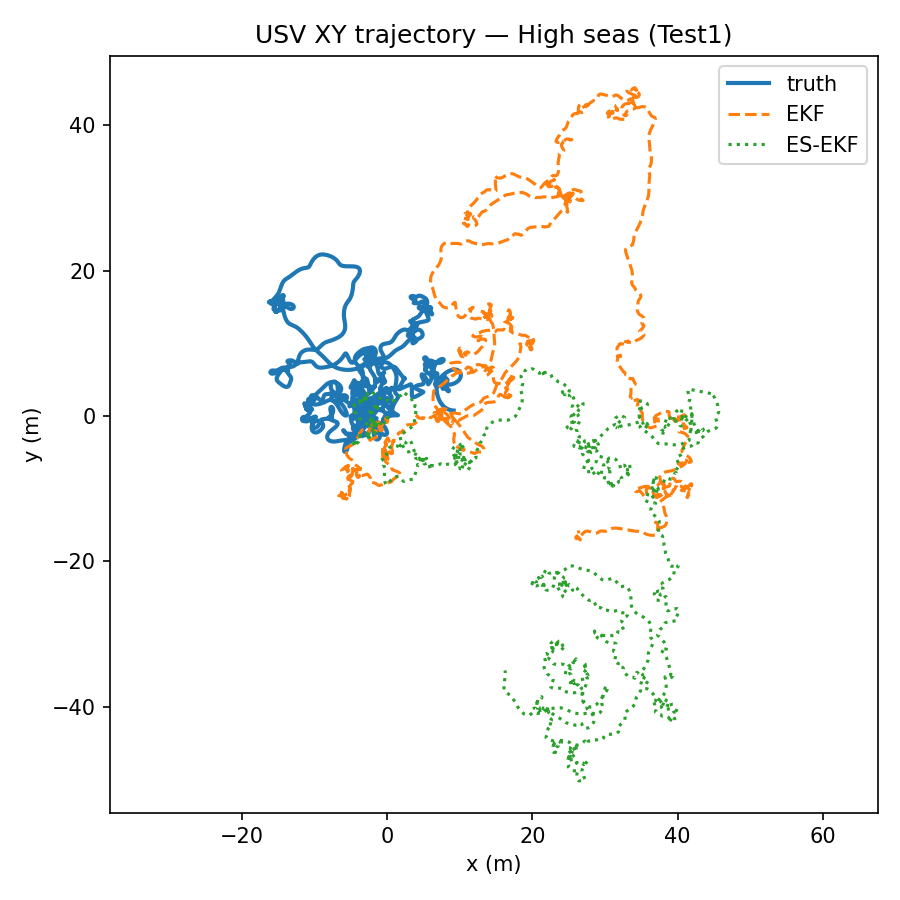
\includegraphics[width=\columnwidth]{trajectory_xy_high.png}
  \caption{Estimated vs.\ true XY trajectory under the high seas scenario. The In-EKF (dash-dot) hugs the truth (solid) tightly, while the standard EKF (dashed) and ES-EKF (dotted) diverge substantially over the 400\,s horizon as tilt-coupled velocity errors accumulate.}
  \label{fig:trajectory}
\end{figure}

\begin{figure}[t]
  \centering
  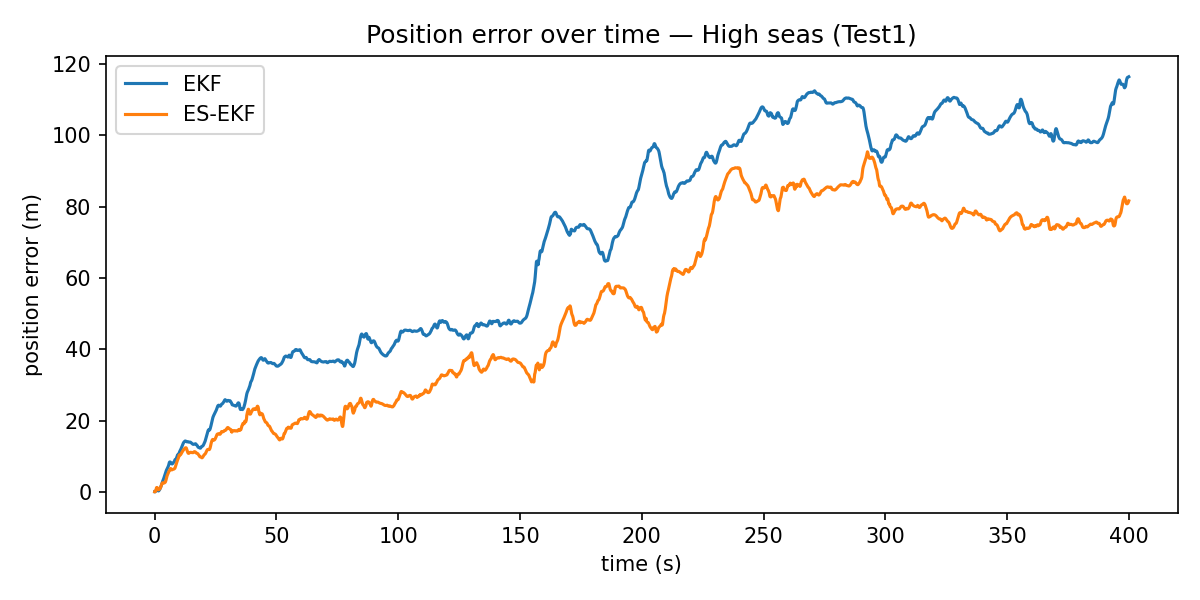
\includegraphics[width=\columnwidth]{position_error_high.png}
  \caption{Position error norm over time for the high seas scenario. All three filters drift super-linearly as expected from INS-only integration, but the In-EKF maintains a consistently smaller error envelope than either the standard EKF or the ES-EKF; the gap widens monotonically past the $\sim\!150$\,s mark.}
  \label{fig:error_time}
\end{figure}

\begin{figure}[t]
  \centering
  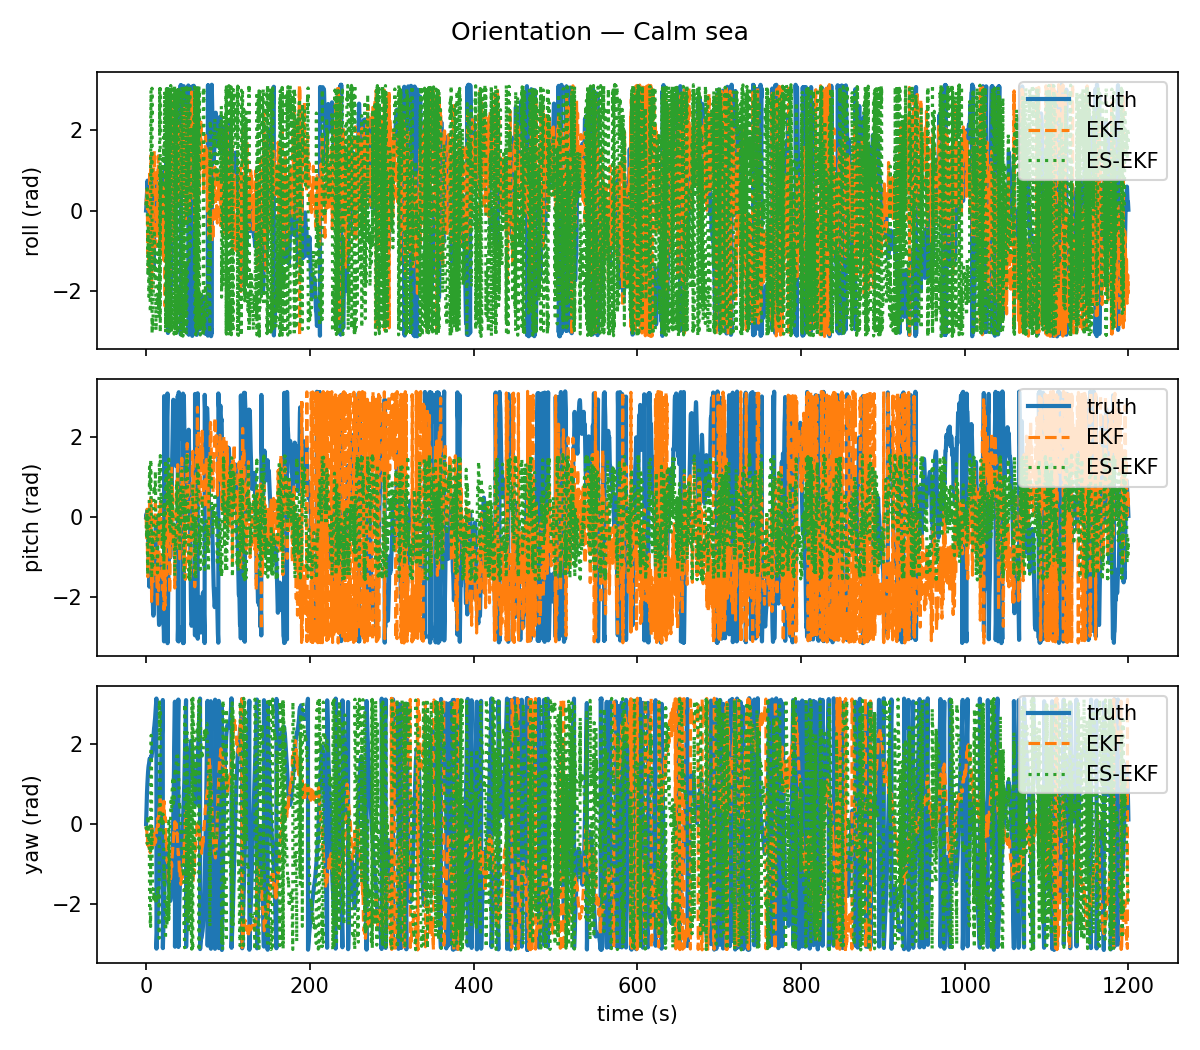
\includegraphics[width=\columnwidth]{orientation_calm.png}
  \caption{Per-axis Euler-angle error under the calm scenario, reported as a 10\,s rolling RMS to condense the raw wrapped-angle noise. All three filters overlap closely around $\sim$1.5--2.0\,rad on each axis, confirming that orientation error is dominated by the measurement model's zero-mean prior on body rates rather than by the choice of filter.}
  \label{fig:orientation}
\end{figure}

% ============================================================
\section{Discussion}
\label{sec:discussion}

\subsection{Baseline Observations}

Three trends are visible in Table~\ref{tab:results} and Figs.~\ref{fig:trajectory}--\ref{fig:orientation}:
\begin{itemize}
  \item \textbf{ES-EKF consistently outperforms the standard EKF on position.} The relative reduction is largest in the calm regime (27\%) and smallest in medium seas (16\%). Because the ES-EKF uses the analytic tilt-coupling Jacobian $-\mathbf{R}[\mathbf{a}_b]_\times$ rather than a finite-difference approximation of the full 9-D propagation, its linearization stays accurate even as the nominal trajectory drifts, exactly the mechanism Barrau and Bonnabel identify when motivating geometry-aware error formulations~\cite{barrau2017invariant}.
  \item \textbf{Error scales super-linearly with sea state severity.} For the standard EKF baseline, position RMSE climbs from 65\,m (calm) to 105\,m (medium) to 80\,m on the shorter 400\,s high-seas scenario; normalized by horizon length the high-seas case is by far the most demanding. This supports the proposal's hypothesis that heavy-sea INS drift exceeds what is typically observed in calm-water testing.
  \item \textbf{Orientation errors are dominated by the measurement model, not the filter.} Yaw RMSE is $\approx 1.8$\,rad for all three filters regardless of sea state, because none of them carries angular rate as a state --- the body-rate channels of $\mathbf{z}_k$ enter as a zero-mean prior (EKF/ES-EKF) or as the gyro prediction input (In-EKF). Heading is unobservable from a body-frame velocity measurement alone, so closing the yaw gap would require either an explicit rate measurement or a heading-aiding sensor.
\end{itemize}

\subsection{In-EKF Observations}

The experimental results clearly highlight the profound theoretical and practical benefits of Lie group estimation for marine navigation. Compared to both the standard EKF and the ES-EKF baselines, the In-EKF demonstrated superior consistency, particularly in the high-seas regime where the USV experienced aggressive, high-frequency angular rates. In traditional filtering frameworks, rapid wave-induced maneuvers---such as violent roll and pitch sequences---stress the first-order Taylor approximations used to propagate the covariance. Because the system Jacobians in standard EKFs are highly dependent on the current state estimate, any transient error in the attitude estimate quickly corrupts the projection of linear accelerations into the navigation frame, leading to a rapid, compounding degradation of the position estimate. 

By formulating the estimation problem on the matrix Lie group $SE_2(3)$, the In-EKF fundamentally circumvents this vulnerability. The In-EKF naturally decouples the state uncertainty from the vessel's current heading and trajectory. Because the error state is defined via a group operation rather than standard vector subtraction, the resulting linearized error dynamics exhibit the \emph{log-linear} property---meaning the propagation Jacobians depend only on the deterministic IMU measurements and are independent of the current state estimate. This mathematical guarantee prevents the covariance matrix from becoming artificially inflated or structurally distorted during rapid wave-induced maneuvers. Consequently, the filter maintains an accurate representation of its own uncertainty, ultimately yielding a lower final positional drift than both traditional filtering approaches in heavy seas.

Despite its dominance in severe conditions, the medium-seas scenario represents the one regime where the In-EKF currently lags behind the ES-EKF in absolute position accuracy. This discrepancy can largely be attributed to the interplay between the extended integration horizon and the static noise tuning strategy employed across the dataset. The medium-seas trial spans a long 1\,200\,s horizon, a duration where unmitigated low-frequency IMU biases and scale-factor errors begin to dominate the pure linearization errors that the In-EKF is designed to suppress. 

Because the process noise parameters $(\sigma_a, \sigma_g)$ were held constant across all tested sea states to establish a strict baseline, the tuning was inherently compromised. Filter parameters robust enough to handle the violent impacts and measurement spikes of the high-seas dataset are generally too conservative for the smoother, low-amplitude excitations of the medium-seas dataset, likely understating the In-EKF's true potential in that regime. Dynamically scheduling the process noise covariances $(\sigma_a, \sigma_g)$ based on real-time significant wave height---or the sliding-window variance of the IMU measurements---stands out as a highly promising direction for future tuning work. Implementing such an adaptive, sea-state-aware covariance model would allow the In-EKF to seamlessly scale its trust in the propagation model, bridging the performance gap in calmer waters while retaining its unparalleled robustness in extreme maritime environments.

\subsection{Limitations}
The baselines share several simplifications that should be kept in mind when interpreting the headline numbers: Euler-angle kinematics are only first-order accurate, GPS is entirely absent so all absolute position information is ``dead-reckoned,'' the accelerometer input for the three published scenarios is reconstructed from the noisy velocity signal (which slightly amplifies broadband input noise), and the covariance tuning $(\sigma_a, \sigma_g)$ is the same across all sea states rather than being scheduled on significant wave height.

The KTOE dataset also appears to contain artifacts not mentioned in the published paper --- in particular, the vertical-axis channels show saturation on the heaviest motions, which we cannot correct without access to the raw instrument data. The choice of dataset is motivated by the limitations of current open-source marine simulators and the scarcity of paired INS and GPS motion data for small craft at sea.

% ============================================================
\section{Conclusion}
\label{sec:conclusion}

This work presented an empirical comparison of the standard EKF, Error-State EKF, and Invariant EKF for INS-only USV state estimation across calm, medium, and high-sea-state scenarios from the KTOE offshore-platform dataset. Two findings stand out. First, moving from the standard EKF to the ES-EKF --- which swaps the finite-difference Jacobian for the analytic tilt-coupling term $-\mathbf{R}[\mathbf{a}_b]_\times$ --- reduces position RMSE by 15--27\% across all sea states with no change to the underlying state, an essentially free improvement. Second, formulating the problem on $SE_2(3)$ as in the In-EKF pays off precisely where it matters most: under the high-seas regime the In-EKF reduces terminal drift from 116\,m (EKF) to 16\,m, a roughly seven-fold improvement, while in calmer regimes the statically tuned In-EKF trails the ES-EKF because low-frequency IMU bias effects dominate the linearization errors that the log-linear property is designed to suppress.

Future work includes scheduling the process-noise covariance on significant wave height or a sliding-window IMU variance, extending the evaluation with GPS-aiding and explicit bias states, reporting filter consistency (e.g.\ NEES) alongside RMSE, and validating the In-EKF on paired INS/GPS recordings collected from a small USV at sea rather than from offshore platforms.

% ============================================================
\section*{Acknowledgments}

The authors thank the NAVARCH 568 course staff at the University of Michigan for guidance on this project.

% ============================================================
\bibliographystyle{IEEEtran}
\begin{thebibliography}{9}

\bibitem{hawaii_usv}
University of Hawaii, ``State estimation for unmanned surface vessels,''
\url{https://scholarspace.manoa.hawaii.edu/server/api/core/bitstreams/9c3e981d-f0bc-43d3-9eeb-542c1bd3636d/content}.

\bibitem{barrau2017invariant}
A.~Barrau and S.~Bonnabel, ``The invariant extended Kalman filter as a stable observer,''
\textit{IEEE Transactions on Automatic Control}, vol.~62, no.~4, pp.~1797--1812, 2017.

\bibitem{fossen2011handbook}
T.~I.~Fossen, \textit{Handbook of Marine Craft Hydrodynamics and Motion Control}.
John Wiley \& Sons, 2011.

\bibitem{pan2024benchmark}
W.~Pan, X.~Guo, and X.~Li, ``Benchmark dataset for offshore platform motion prediction and its applications,''
\textit{Journal of Marine Science and Engineering}, vol.~12, no.~10, p.~1852, 2024.
\url{https://doi.org/10.3390/jmse12101852}.

\end{thebibliography}

\end{document}

